% LipScribe -- Progress Report 4 (Week 4: beyond GRID, decoding, demo, and the TED plan)
% Compile: latexmk -pdf progress_report_week4.tex   (or pdflatex twice)
\documentclass[11pt,a4paper]{article}
\usepackage{lipscribe-report}
\usepackage{graphicx}
\usepackage{amsmath}
\usepackage{float}
\usepackage{tikz}
\usetikzlibrary{arrows.meta,positioning,shapes.geometric}
\fancyhead[L]{\small\sffamily\color{lsgrey}LipScribe -- Progress Report 4 (Week 4: Beyond GRID)}

\newcommand{\code}[1]{\texttt{\small #1}}
% \tile{big number}{explanation}
\newcommand{\tile}[2]{\colorbox{lslight}{\parbox[t][1.55cm][t]{0.212\textwidth}{\sffamily\raggedright
  {\Large\bfseries\color{lsblue}#1}\par\vspace{3pt}{\scriptsize\linespread{1.0}\selectfont #2\par}}}}
% a shaded "key idea" box for the reader
% (parfillskip=0pt: the style's parskip[parfill] keeps 30pt free at the end of a paragraph,
%  which would push a full-width box past the margin)
\newcommand{\keyidea}[2]{\par\smallskip{\parfillskip=0pt\noindent\colorbox{lsrow}{\parbox{\dimexpr\linewidth-2\fboxsep}{\small
  {\sffamily\bfseries\color{lsblue}Key idea -- #1.}\enspace #2}}\par}\smallskip}
\newcolumntype{L}[1]{>{\raggedright\arraybackslash}p{#1}}
\setlength{\textfloatsep}{10pt plus 2pt minus 2pt}
\setlength{\floatsep}{8pt plus 2pt minus 2pt}
\setlist{itemsep=1pt,topsep=2pt,parsep=0pt}

\begin{document}

\docheader{Progress Report 4}{Week 4: Testing Model~P Beyond GRID, Decoding, a Live Demo, and the TED Training Plan}{12 November 2026}

% =====================================================================
\section{Summary}
By the end of Week~3 (report of 9~November) LipScribe worked very well \emph{inside} the GRID
corpus. Model~P4 got $1.02\,\%$ of test words wrong on clean speech and $0.71\,\%$ with grammar
decoding. In Week~4 we asked the harder question an examiner would ask: \textbf{does it work
outside GRID?} This report covers four strands of work:

\begin{enumerate}
  \item \textbf{Understanding and presenting the GRID system.} We measured exactly what grammar
  decoding contributes: on P4's test set it fixed 555 sentences and made none worse. We built
  a 23-slide progress presentation for a non-specialist audience, merged the first caption
  application (PR~\#55), and built a browser demo that records a clip and captions it on our
  GPU workstation.
  \item \textbf{A first out-of-domain test (``Flix'').} We built a pipeline that finds moments
  in films and TV where one person faces the camera and speaks. It crops their mouth exactly as
  we did for GRID and labels the clip with the subtitle. Model~P, which knows only GRID's
  51 words, got essentially \emph{every} film word wrong, and so did every retrained version.
  The experiment still taught us a lot. Letter accuracy improved steadily as data grew, and an
  open-vocabulary ``word grammar'' produced real words for the first time. The clear lesson is
  that \textbf{data, not architecture, is now our limit}.
  \item \textbf{More data, done properly.} We scaled the data by more than 100 times during
  the week. Films without subtitles were labelled automatically with a speech recogniser
  (Whisper), and we harvested 3,040 TED talks. TED talks are a licensed source with
  professional transcripts, the same source as the standard LRS3 lip-reading benchmark. Each
  talk is downloaded, mined and deleted, so only mouth crops are kept.
  \item \textbf{A rigorous training plan on that data}, now running on the Alienware. It will
  try all 11 ways of training the visual encoder (ResNet-18) for 60 epochs each, then train the
  winner three times, and score it on films and on held-out TED talks.
\end{enumerate}

\medskip
\noindent\tile{0.71\,\%}{P4 + GRID grammar, clean test WER; 555 sentences fixed, 0 broken}\hfill%
\tile{$>$100$\times$}{growth in labelled out-of-domain speech this week (8 min $\rightarrow$ 21 h)}\hfill%
\tile{96.3\,\%}{best film-test WER so far (v2 + word grammar): honest, and data-limited}\hfill%
\tile{2--3\,s}{live demo: browser recording $\rightarrow$ caption on the Alienware}

% =====================================================================
\section{The Journey So Far (Weeks 1--4)}
Table~\ref{tab:journey} is the short version of the whole project. The milestone dates are
those of our project plan.

\begin{table}[htbp]
\centering\small
\caption{What we have built, week by week.}
\label{tab:journey}
\rowcolors{2}{lsrow}{white}
\begin{tabularx}{\textwidth}{@{}L{1.5cm}X@{}}
\toprule
\rowcolor{white}\sffamily\bfseries Week & \sffamily\bfseries What we achieved \\
\midrule
Week 1 & Environment on the Alienware (RTX~4080 SUPER, 16\,GB). GRID corpus (33 speakers,
32,890 clips) and MUSAN noise verified; speaker-independent split (26 train / 3 val / 4 test). \\
Week 2 & Preprocessing: MediaPipe Face Mesh mouth crops ($96{\times}96$ grey, 25\,fps), audio
re-aligned to the lips (silence had been trimmed), corpus audit, fixed noisy test sets at
5 noise levels, shared \code{GridDataset}. \\
Week 3 & Baselines B1 (ears), B2 (eyes; Conv3D and ResNet-18), B3 (simple fusion); evaluation
engine; CTC beam search and GRID grammar decoder; Model~P (cross-modal attention, gated
fusion, missing-modality embedding) with four initialisations. \textbf{P4: 1.02\,\% WER clean.} \\
Week 4 & Grammar analysis; MFCC audio-feature experiment (W3-08); caption app (PR~\#55);
progress presentation; web demo; the out-of-domain experiment (films, Whisper, TED); a
data pipeline that is now harvesting $\sim$27\,h of labelled lip clips; the v3 training plan. \\
\bottomrule
\end{tabularx}
\end{table}

{\small
\rowcolors{2}{lsrow}{white}
\begin{tabularx}{\textwidth}{@{}XL{1.9cm}L{7.4cm}@{}}
\toprule
\rowcolor{white}\sffamily\bfseries Milestone & \sffamily\bfseries Due & \sffamily\bfseries Status \\
\midrule
M1 Environment and dataset & Sun 25 Oct & \done{} -- closed 29 Oct \\
M2 Preprocessing and alignment & Sun 1 Nov & \done{} -- closed 3 Nov \\
M3 \& M4 Baselines B1, B2, B3 & Sun 8 Nov & \done{} -- closed 4 Nov \\
M5 Multimodal fusion (Model P) & Sun 15 Nov & \done{} -- P1--P4 trained and tested \\
M6 \& M7 Tuning and evaluation & Sun 22 Nov & \inprog{} -- grammar analysis, X6 out-of-domain test and ResNet tuning done; v3 running \\
M8 \& M9 Application, testing, demo & Sun 29 Nov & \inprog{} -- caption app merged; browser demo working end to end \\
\bottomrule
\end{tabularx}
}

% =====================================================================
\section{Growth Since the Week 3 Report}
\label{sec:growth}
The Week~3 report ended with two next steps: gate and attention visualisation (W4-06), and
ablations plus application integration (W4-07--W4-10). Table~\ref{tab:growth} shows how far the
project moved in three days.

\begin{table}[htbp]
\centering\small
\caption{Week 3 report (9 Nov) compared with today (12 Nov).}
\label{tab:growth}
\rowcolors{2}{lsrow}{white}
\begin{tabularx}{\textwidth}{@{}L{3.2cm}XX@{}}
\toprule
\rowcolor{white}\sffamily\bfseries Area & \sffamily\bfseries Week 3 report & \sffamily\bfseries Now (Week 4) \\
\midrule
Scope of testing & GRID only (51-word vocabulary, studio recordings) & GRID \emph{and} films, TV, TED: open vocabulary, real lighting, real camera work \\
Decoding & Greedy and GRID grammar reported side by side & Grammar effect quantified per sentence (555 fixed, 0 broken); new open-vocabulary \emph{word grammar} (word list + bigram language model) \\
Audio features (W3-08) & Planned & Done by Lisa and Charis: adding MFCC to log-Mel lowered ears-only validation error from 7.7\,\% to 6.9\,\% (branch \code{charis}, not yet merged) \\
Application (W3-10) & Gradio skeleton in progress & Caption app merged (PR~\#55, 10 Nov); browser demo (\code{demo/}) captions a phone recording in 2--3\,s \\
Training data & 26 GRID speakers ($\approx$27\,h) & + 1,268 film clips, 1,016 Whisper-labelled film clips, $\sim$29,000 TED clips (21\,h so far) \\
Visual encoder & ResNet-18 chosen over Conv3D (P3 vs P4) & 11 ways of training the ResNet compared; fine-tuning it at 0.3$\times$ the learning rate wins on films \\
Infrastructure & Manual runs & Resumable chain with automatic restart after a reboot; download--mine--delete harvester \\
Communication & Technical report & 23-slide presentation for non-specialists, with real scenes and training logs \\
\bottomrule
\end{tabularx}
\end{table}

% =====================================================================
\section{GRID: What Grammar Decoding Really Does}
\label{sec:grammar}
\keyidea{decoding}{Twenty-five times a second the model outputs a probability for every letter
(and a ``gap'' symbol). \emph{Decoding} turns that stream into words. \textbf{Greedy} decoding
takes the most likely letter at each moment, merges repeats and drops the gaps. It is fast,
but one weak letter spells a wrong word. A \textbf{grammar} decoder only allows sentences that
fit a pattern and picks the allowed sentence that best matches the letter probabilities.}

Every GRID sentence has six slots, \emph{command--colour--preposition--letter--digit--adverb},
drawn from 51 words. Comparing P4's per-sentence outputs with and without the grammar on all
19,990 test sentence/noise pairs:
\textbf{555 sentences were corrected and none were made worse}. Real examples at 0\,dB include
\emph{``place white by x five \textbf{snow}''} $\rightarrow$ \emph{``\ldots five \textbf{now}''}
and \emph{``lay red by k \textbf{ninhe} please''} $\rightarrow$ \emph{``\ldots k \textbf{nine} please''}.
Errors fall by 30\,\% in a quiet room ($1.02 \rightarrow 0.71\,\%$) and 26\,\% in the noisiest
($5.34 \rightarrow 3.95\,\%$).

{\small
\rowcolors{2}{lsrow}{white}
\begin{tabularx}{\textwidth}{@{}Xccccc|c@{}}
\toprule
\rowcolor{white}\sffamily\bfseries Model P4, test WER \% & \textbf{Clean} & \textbf{10 dB} & \textbf{5 dB} & \textbf{0 dB} & \textbf{$-$5 dB} & \textbf{Mean} \\
\midrule
Greedy & 1.02 & 1.53 & 1.87 & 2.79 & 5.34 & 2.51 \\
GRID grammar & \textbf{0.71} & \textbf{1.10} & \textbf{1.42} & \textbf{2.06} & \textbf{3.95} & \textbf{1.85} \\
\bottomrule
\end{tabularx}
}

The grammar only works because GRID is artificial. Real speech has no fixed pattern, which is
why the out-of-domain work below needed a different decoder (Section~\ref{sec:lm}).

% =====================================================================
\section{Experiment X6 ``Flix'': Does Model P Work Outside GRID?}
\label{sec:flix}
\keyidea{domain shift}{A model learns the statistics of its training data. GRID is one
person, facing the camera, in a studio, saying six words from a 51-word list. Films have
other faces, lighting, head turns, camera cuts and \emph{any} English word. Testing on data
that differs from the training data is called \emph{out-of-domain} evaluation. It is the
honest test of whether a model generalises.}

\subsection{Building the film dataset}
We wrote \code{scripts/mine\_flix.py}, which turns subtitled films and series into clips that
are \emph{identical in format} to GRID's (Figure~\ref{fig:pipeline}). The crop step calls the
same functions as GRID preprocessing (\code{lipscribe.preprocessing.crop}). The test titles
(\emph{Challengers}, \emph{Little Women}, \emph{The Drama}) are never used for training, just
as GRID test speakers never are.

\begin{figure}[htbp]
\centering
\begin{tikzpicture}[node distance=3mm, every node/.style={font=\scriptsize\sffamily},
  box/.style={draw=lsblue, fill=lslight, rounded corners=2pt, align=center, minimum height=11mm, text width=17.6mm},
  rej/.style={draw=red!60!black, fill=red!6, rounded corners=2pt, align=center, text width=17.6mm, minimum height=7mm},
  ar/.style={-{Stealth[length=2mm]}, lsblue, thick}]
\node[box] (a) {Subtitle line\\0.8--3\,s (TED: 5\,s)};
\node[box, right=of a] (b) {Decode frames\\at 25\,fps};
\node[box, right=of b] (c) {Exactly one\\large, frontal\\face?};
\node[box, right=of c] (d) {Lips move?\\no camera cut?};
\node[box, right=of d] (e) {$96{\times}96$ mouth\\crops + 16\,kHz\\audio + text};
\node[box, right=of e, fill=lsdone!15, draw=lsdone] (f) {Same format\\as GRID\\{\tiny\texttt{GridDataset}}};
\draw[ar] (a) -- (b); \draw[ar] (b) -- (c); \draw[ar] (c) -- (d); \draw[ar] (d) -- (e); \draw[ar] (e) -- (f);
\node[rej, below=4mm of c] (r1) {reject: no face,\\2 faces, profile};
\node[rej, below=4mm of d] (r2) {reject: cut,\\still lips};
\draw[ar, red!60!black] (c) -- (r1); \draw[ar, red!60!black] (d) -- (r2);
\end{tikzpicture}
\caption{The clip-mining pipeline used for films, Whisper-labelled films and TED talks. About
7--8\,\% of subtitle lines survive the filters; the rest show slides, the audience, two
people, a turned head or a camera cut.}
\label{fig:pipeline}
\end{figure}

\begin{figure}[htbp]
\centering
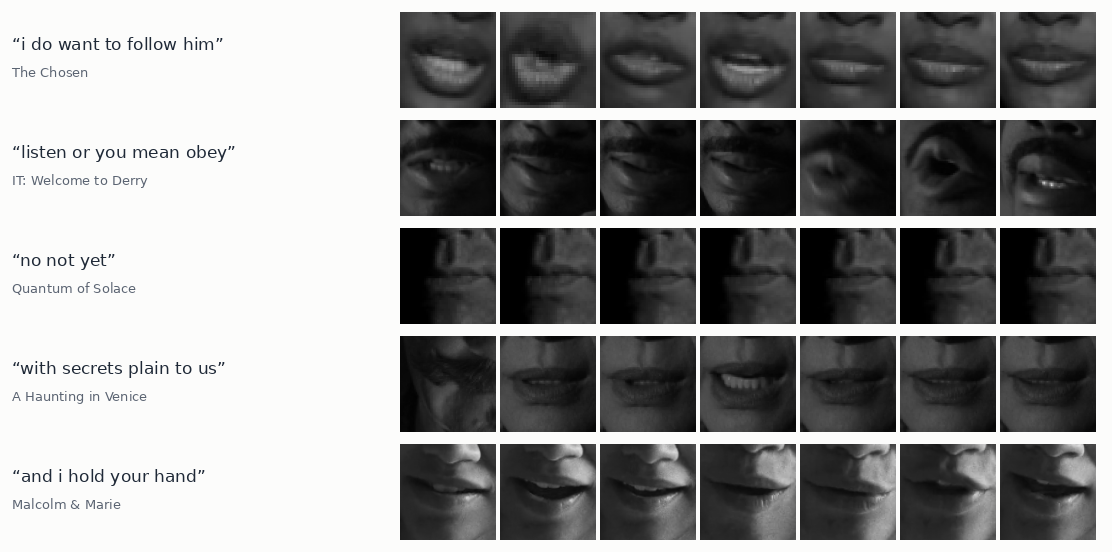
\includegraphics[width=0.78\textwidth]{figures/film_mouths.png}
\caption{Real mouth crops found by the miner (7 moments per line) with the subtitle that labels
them. Note how much more varied the lighting and pose are than in GRID's studio clips.}
\label{fig:mouths}
\end{figure}

The first mining run (capped at 220 lines per film and 45 per episode) kept \textbf{305 clips:
9.7 minutes of speech containing 651 different words}, compared with GRID's 51.

\subsection{Three ways of using the data}
\begin{enumerate}
  \item \textbf{Fine-tune P4 with GRID mixed in.} Continue training a \emph{copy} of P4 on
  film clips plus 1,000 GRID clips, so it does not forget GRID. The main checkpoint
  \code{p\_proposed\_best.pt} is never written; every report records its unchanged MD5 checksum.
  \item \textbf{Retrain the P4 way on films only.} Start from the trained B1 ears and B2 eyes
  with a new fusion layer and output head, exactly as P4 was built. A 26-setting
  hyperparameter sweep chose the best setting (learning rate $10^{-3}$, eyes frozen, batch 8,
  mostly clean audio). We then trained that setting three times (seeds 1--3) for 150 epochs to
  measure the spread.
  \item \textbf{Add a word grammar} (Section~\ref{sec:lm}) on top of the retrained model.
\end{enumerate}

\keyidea{why we chose models by CER, not WER}{On film speech nearly every \emph{word} is wrong
($\approx$100\,\% WER), so WER cannot tell two models apart. The character error rate (CER)
still moves, because a model that writes ``trusk'' for ``trust'' is closer than one that writes
``bin''. We therefore selected checkpoints by validation CER. We also enlarged the validation
set from 18 to 69 clips, by moving two training titles into it, because tuning on 18 clips
mostly measures luck.}

\subsection{Results}
Table~\ref{tab:flix} and Figure~\ref{fig:flix} use the same 43 test clips from three films that
none of the models ever saw. Rows marked ``mean of 3'' are averaged over three seeds.

\begin{table}[htbp]
\centering\small
\caption{Film test (43 clips, 3 unseen films, clean sound). WER/CER in \%. ``New words'' =
non-GRID words written correctly, out of 223.}
\label{tab:flix}
\rowcolors{2}{lsrow}{white}
\begin{tabularx}{\textwidth}{@{}Xcccc@{}}
\toprule
\rowcolor{white}\sffamily\bfseries Model & \textbf{WER} & \textbf{CER} & \textbf{New words} & \textbf{GRID test WER} \\
\midrule
P4 as is (no film training) & 109.2 & 81.5 & 2 & 0.8 \\
P4 fine-tuned with GRID mixed in & 102.0 & 77.9 & 2 & 2.8 \\
v1: retrained on 193 film clips (mean of 3) & 103.1 & 74.5 & $\approx$3 & 115 \\
v2: retrained on 1,156 film clips (mean of 3) & 103.2 & \textbf{72.5} & $\approx$2 & 116 \\
v2 + word grammar (mean of 3) & \textbf{96.3} & 78.9 & \textbf{$\approx$7} & -- \\
\bottomrule
\end{tabularx}
\end{table}

\begin{figure}[htbp]
\centering
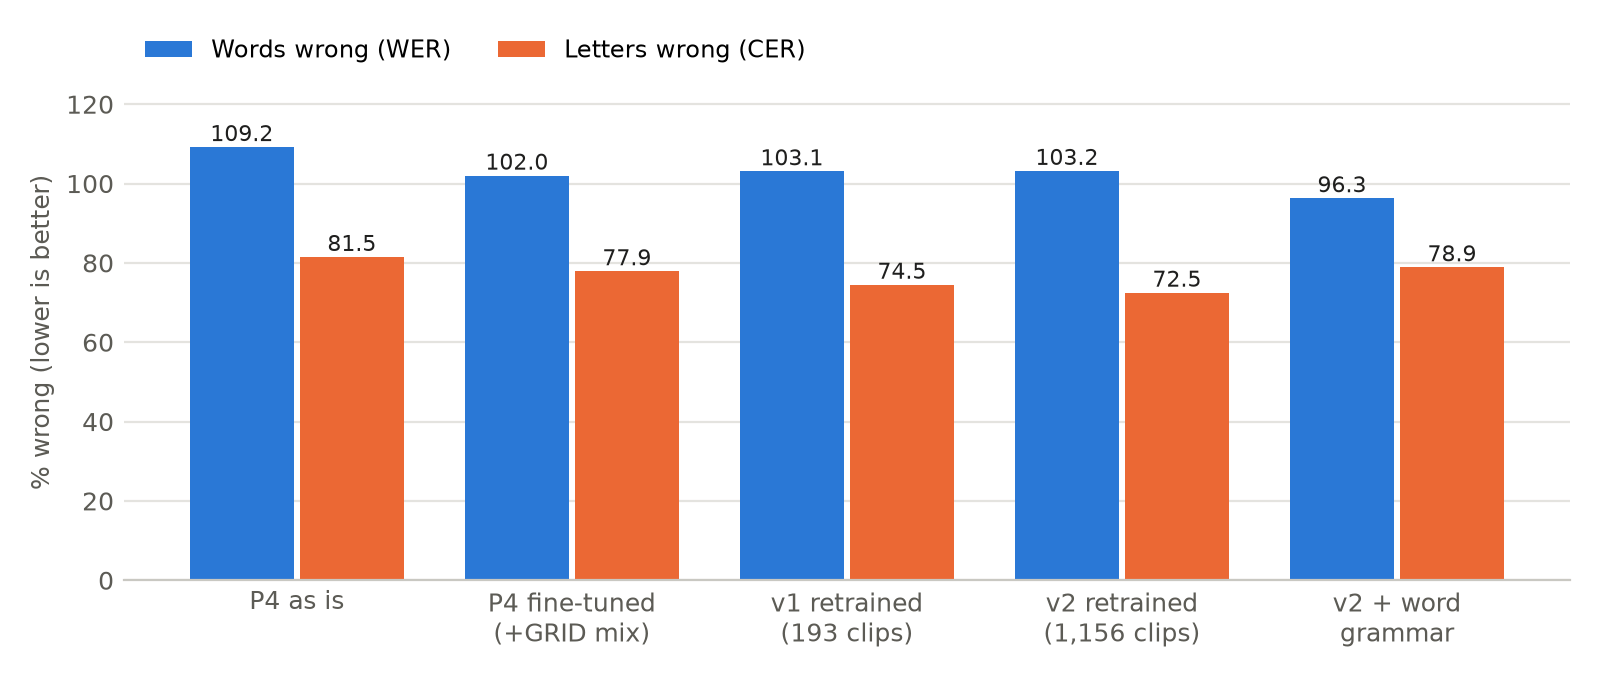
\includegraphics[width=0.86\textwidth]{figures/fig_flix_results.png}
\caption{Words and letters wrong on the film test. WER can exceed 100\,\% when the model adds
words. Letters improve as data grows; the word grammar is the first to bring WER below 100\,\%.}
\label{fig:flix}
\end{figure}

\paragraph{How to read these results.}
\begin{itemize}
  \item \textbf{Letters improve with data.} CER falls from 81.5\,\% to 74.5\,\% (v1) and then to
  72.5\,\% (v2, six times more clips). The three seeds agree within $\approx$1--2 points, so the
  trend is real.
  \item \textbf{Words do not improve yet.} Even v2 has heard only $\approx$37 minutes of film
  speech. Published open-vocabulary lip-readers train on hundreds of hours.
  \item \textbf{Forgetting.} Trained on films only, the retrained models lose GRID completely
  (0.8\,\% $\rightarrow$ 115\,\% WER). This is \emph{catastrophic forgetting}. Mixing GRID into
  the training data (row 2) prevents it, at a small cost (2.8\,\%).
  \item \textbf{Lips vs sound.} With the sound muted, the retrained models do worse (CER
  $\approx$88--91\,\%). The winning setting froze the eyes, so the model learned to rely on the
  audio. The ResNet tuning below revisits this.
\end{itemize}

\begin{figure}[htbp]
\centering
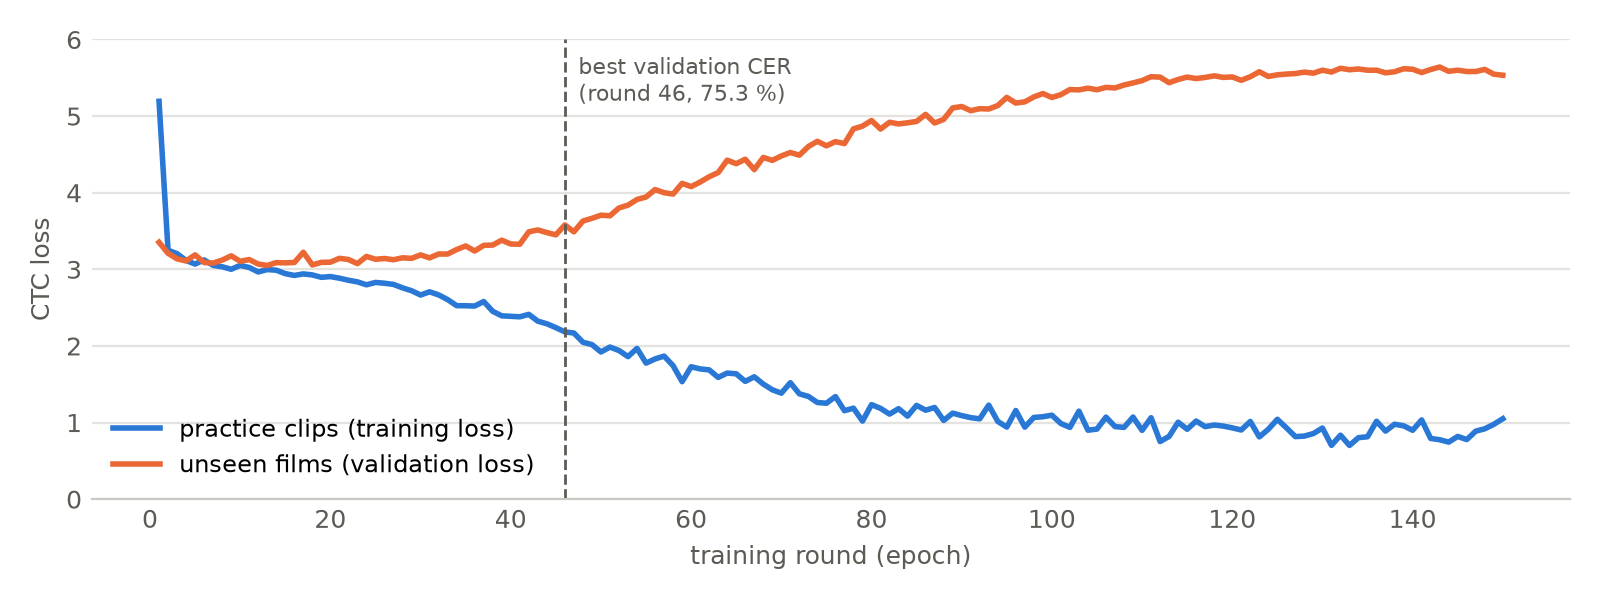
\includegraphics[width=0.86\textwidth]{figures/fig_training_curve.png}
\caption{Overfitting, seen directly (v1, seed 1, 150 epochs). The loss on the 193 training
clips keeps falling, while the loss on unseen films starts rising after about round 10. The
best validation CER came at round 46. We keep that checkpoint, not the last one.}
\label{fig:curve}
\end{figure}

\begin{table}[htbp]
\centering\small
\caption{Excerpt from the real training log of the same run (Alienware). ``Error'' is the CTC
loss; letters wrong is the validation CER on unseen films.}
\label{tab:log}
\rowcolors{2}{lsrow}{white}
\begin{tabular}{@{}rccc@{}}
\toprule
\rowcolor{white}\sffamily\bfseries Round & \sffamily\bfseries Practice error & \sffamily\bfseries Unseen-film error & \sffamily\bfseries Letters wrong \\
\midrule
1   & 5.19 & 3.35 & 100.0\,\% \\
10  & 3.05 & 3.10 & 100.0\,\% \\
30  & 2.66 & 3.19 & 86.4\,\% \\
\textbf{46} & 2.18 & 3.58 & \textbf{75.3\,\%} (best, kept) \\
100 & 1.10 & 5.24 & 78.3\,\% \\
150 & 1.05 & 5.53 & 78.5\,\% \\
\bottomrule
\end{tabular}
\end{table}

Two things stand out in Table~\ref{tab:log}. For the first $\sim$30 rounds the letters-wrong
column stays at 100\,\%. That is the new CTC head writing only gaps, the behaviour that forced us
to raise the early-stopping patience. After round 46 the practice error keeps falling while the
model gets worse on unseen films: the textbook signature of overfitting.

\keyidea{overfitting}{When a model has many more parameters than examples, it can memorise the
training set. Figure~\ref{fig:curve} shows the signature: training error falls while error on
unseen data rises. The cures are more data, more augmentation, stronger regularisation, and
stopping at the best validation point. This is exactly what the TED plan (Section~\ref{sec:ted})
is designed around.}

\subsection{An open-vocabulary ``word grammar''}
\label{sec:lm}
For films we wrote \code{lipscribe/decoding/lexicon\_lm.py}, a CTC beam search with two
constraints:
\begin{itemize}
  \item a \textbf{lexicon}: a partial word may only grow along a tree of known words, so every
  output word is a real word;
  \item a \textbf{bigram language model}, which scores each finished word by how likely it is to
  follow the previous one.
\end{itemize}
Both were built from \textbf{every subtitle line of the training films only}: 23,455 lines,
141,687 words and a 9,053-word lexicon. Validation and test films were excluded, so the test
stays honest. 95\,\% of the words actually spoken in the test films are in the lexicon. The LM
weight and a word bonus were tuned on validation, and the test was scored once. The word
grammar roughly tripled the number of correct non-GRID words and gave the first sub-100\,\% WER.
Figure~\ref{fig:scenes} shows what this looks like.

\begin{figure}[htbp]
\centering
\noindent\begin{minipage}[c]{0.43\textwidth}
\includegraphics[width=\linewidth]{figures/strip_1.png}\end{minipage}\hfill
\begin{minipage}[c]{0.54\textwidth}\footnotesize
{\sffamily\bfseries\color{lsblue}Best result} \textcolor{lsgrey}{(\emph{The Drama})}\\[1pt]
\textbf{Subtitle:} ``you know like uh''\\
\textcolor{lsgrey}{P4 as is:} \texttt{bn ne now}\quad \textcolor{lsgrey}{Retrained:} \texttt{you nt a ne}\\
\textcolor{lsgrey}{Retrained + word grammar:} \textbf{\texttt{you dont and}}
\end{minipage}
\par\medskip
\noindent\begin{minipage}[c]{0.43\textwidth}
\includegraphics[width=\linewidth]{figures/strip_2.png}\end{minipage}\hfill
\begin{minipage}[c]{0.54\textwidth}\footnotesize
{\sffamily\bfseries\color{lsblue}Best result} \textcolor{lsgrey}{(\emph{Little Women})}\\[1pt]
\textbf{Subtitle:} ``i used to be''\\
\textcolor{lsgrey}{P4 as is:} \texttt{lian whe win b eight sgon}\quad \textcolor{lsgrey}{Retrained:} \texttt{wha ma ne}\\
\textcolor{lsgrey}{Retrained + word grammar:} \textbf{\texttt{i am}}
\end{minipage}
\par\medskip
\noindent\begin{minipage}[c]{0.43\textwidth}
\includegraphics[width=\linewidth]{figures/strip_3.png}\end{minipage}\hfill
\begin{minipage}[c]{0.54\textwidth}\footnotesize
{\sffamily\bfseries\color{lsblue}Typical result} \textcolor{lsgrey}{(\emph{Little Women})}\\[1pt]
\textbf{Subtitle:} ``oh i thought you were a novelist not a screenwriter''\\
\textcolor{lsgrey}{P4 as is:} \texttt{lay reten bi v iro soon}\quad \textcolor{lsgrey}{Retrained:} \texttt{iond tao u maes srs sne te}\\
\textcolor{lsgrey}{Retrained + word grammar:} \textbf{\texttt{and to me sense}}
\end{minipage}
\caption{Captions generated on the unseen test films. On the left are the mouth crops the model
actually read for the line (7 of its frames); on the right, the real subtitle and the captions of
P4, the retrained model, and the retrained model with the word grammar (seed 1). Two are the best
of the 43 test clips and one is typical.}
\label{fig:scenes}
\end{figure}

The original model forces every film line into a GRID sentence (``\ldots eight soon''). The
retrained model writes English-like fragments, and the word grammar turns some of those into
real words. It is progress, but not yet captioning.


\subsection{Tuning the eyes: 11 ways of training the ResNet}
\keyidea{adopted architecture vs transfer learning}{B2~v2's eyes use the published ResNet-18
lip-reading \emph{design}, but every weight was learned from scratch on GRID: we adopted the
architecture. \emph{Transfer learning} means reusing learned weights. We do that when Model~P
starts from B1 and B2, and when the film models start from GRID-trained encoders. The
question here is how much of the transferred eye to let change.}

On the v2 data we compared 11 variations (Figure~\ref{fig:resnet}): frozen, fine-tuned at
0.1$\times$ or 0.3$\times$ the learning rate, only the top stages trained, only the BiLSTM
trained, and combinations with stronger augmentation, spatial dropout and more frequent video
dropout. \textbf{Fine-tuning the whole ResNet at 0.3$\times$ the learning rate won}
(73.2\,\% validation CER, against 75.0\,\% frozen). So even with about an hour of film speech,
adapting the eyes to film lighting and pose already helps. Gaps of one or two points on 69
validation clips are within noise, which is one reason the TED run repeats all 11 variations
on far more data.

\begin{figure}[H]
\centering
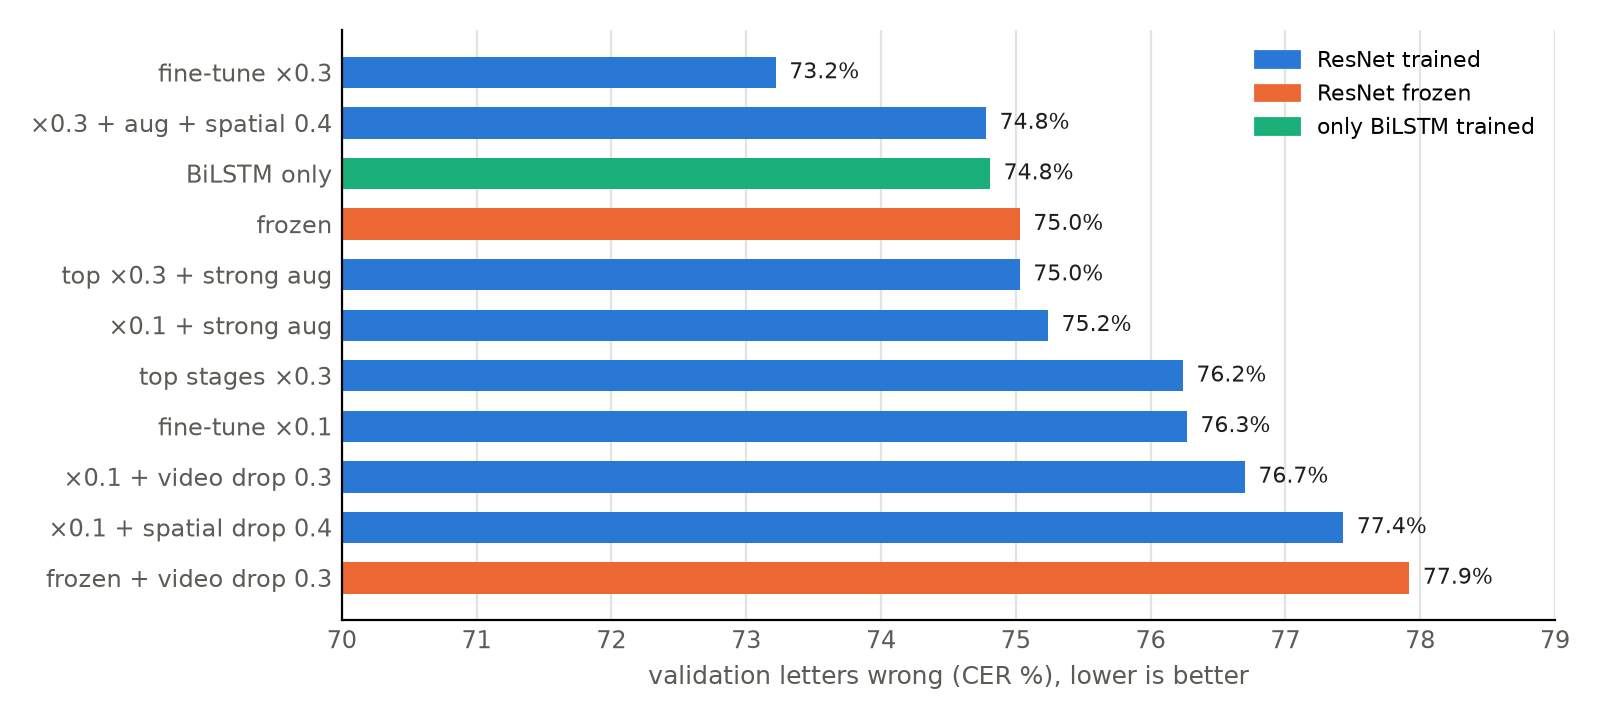
\includegraphics[width=0.86\textwidth]{figures/fig_resnet_tuning.png}
\caption{Validation CER for the 11 eye-training variations on the v2 film data (80 epochs, patience 40).}
\label{fig:resnet}
\end{figure}

% =====================================================================
\section{Setbacks Met Today, and What They Taught Us}
\label{sec:setbacks}
Most of Week~4's out-of-domain work happened on 12~November, and it was not smooth.
Table~\ref{tab:setbacks} lists every significant problem honestly, with its fix. Several are
general engineering lessons rather than lip-reading ones.

{\small
\rowcolors{2}{lsrow}{white}
\begin{longtable}{@{}L{3.3cm}L{4.0cm}L{6.9cm}@{}}
\caption{Setbacks on 12 November, their effect and the fix.}\label{tab:setbacks}\\
\toprule
\rowcolor{white}\sffamily\bfseries Setback & \sffamily\bfseries Effect & \sffamily\bfseries Fix / lesson \\
\midrule
\endfirsthead
\toprule
\rowcolor{white}\sffamily\bfseries Setback & \sffamily\bfseries Effect & \sffamily\bfseries Fix / lesson \\
\midrule
\endhead
Laptop out of memory (03:00, again 14:00) & 4 mining workers on a 7\,GB laptop were killed & 2--3 workers; recycle worker processes; a process pool that \emph{fails loudly} instead of hanging \\
A killed worker hung the whole pool & Mining silently stalled 04:10--06:34 & Switched to \code{ProcessPoolExecutor} plus a 15-minute stall guard. \emph{Lesson:} long jobs need watchdogs \\
Too little data at first & 305 clips (9.7 min) & Mined every subtitle line, then added Whisper and TED (Section~\ref{sec:ted}) \\
WER stuck at $\approx$100\,\% & Could not compare models & Selected by CER; enlarged the validation set from 18 to 69 clips \\
New CTC head outputs only blanks for $\sim$30 epochs & Early stopping killed the P4-recipe runs & Patience 15 $\rightarrow$ 40. \emph{Lesson:} know your loss's warm-up behaviour \\
Overfitting & Best epoch 45 of 150 & Keep the best-validation checkpoint; more data; ResNet and augmentation tuning \\
No \code{ffmpeg} on the Alienware & Could not mine there; a direct binary download was blocked & Pre-extracted 16\,kHz audio on the laptop, decoded video with OpenCV, and used the PyPI \code{imageio-ffmpeg} \\
Network too slow for 58\,GB of video & Relay 0.1\,MB/s, campus 0.4--6\,MB/s & Copied only the 31\,GB the miner uses; mined on the laptop and shipped only clips \\
First 12\,GB copied were cartoons & Unusable (not real lips, no subtitles) & Prioritised a list of useful titles. \emph{Lesson:} check \emph{what} you copy, not just how fast \\
Shell and file-format bugs & \code{ffmpeg} swallowed a loop's input; libsndfile rejected Ogg Opus & \code{ffmpeg -nostdin}; switched to Ogg Vorbis \\
Most TED talks are hosted on YouTube & 97,000 sitemap entries, mostly unusable; we did not bypass YouTube's bot checks & Used TED's 772 playlists: 3,040 TED-hosted talks, all usable \\
TED downloads returned HTTP 404 & Every talk skipped & Fresh download per talk instead of re-using processed metadata \\
Face model missing on the Alienware & TED talks mined to 0 clips & Copied \code{face\_landmarker.task}; added a debug mode that names the filter rejecting each line \\
Python 3.11 pool deadlock & Harvester froze after $\sim$480 lines & Worker recycling only on Python $\ge$ 3.13 \\
Copyright of films & Downloading films automatically would be piracy & Declined; used TED (CC BY-NC-ND, non-commercial academic use, lecturer approval) \\
\bottomrule
\end{longtable}
}

% =====================================================================
\section{The Plan: Training on TED Talks (v3)}
\label{sec:ted}
\subsection{Why TED}
TED talks are close to ideal for lip reading. One speaker faces the camera in good light,
speech is clear, and every talk has professional English subtitles. They are published under
Creative Commons BY-NC-ND for non-commercial use, and they are the source of LRS3, the
standard benchmark for open-vocabulary lip reading. That makes our results comparable in
spirit to published work.

\subsection{How the data is collected}
\code{scripts/ted\_harvest.py} works through the 3,040 talks in TED's playlists, using TED's
own servers only. For each talk it:
\begin{enumerate}
  \item checks that the audio is English and English subtitles exist;
  \item downloads the 640$\times$480 video;
  \item mines every subtitle line of 0.8--5\,s through the same pipeline
  (Figure~\ref{fig:pipeline});
  \item \textbf{deletes the video, audio and subtitles}, keeping only mouth crops, clip audio
  and text.
\end{enumerate}
About 3\,\% of talks (57 so far, 910 clips) are held out as a separate \textbf{TED test set}.
The film validation and test sets never change, so every version stays comparable. Two smaller
sources join TED:
\begin{itemize}
  \item 11 live-action films \emph{without} subtitles, labelled by the Whisper speech
  recogniser (large-v3-turbo, word timings): 1,016 clips;
  \item all remaining subtitle lines of five subtitled training films: 963 more clips (v2).
\end{itemize}

\begin{figure}[htbp]
\centering
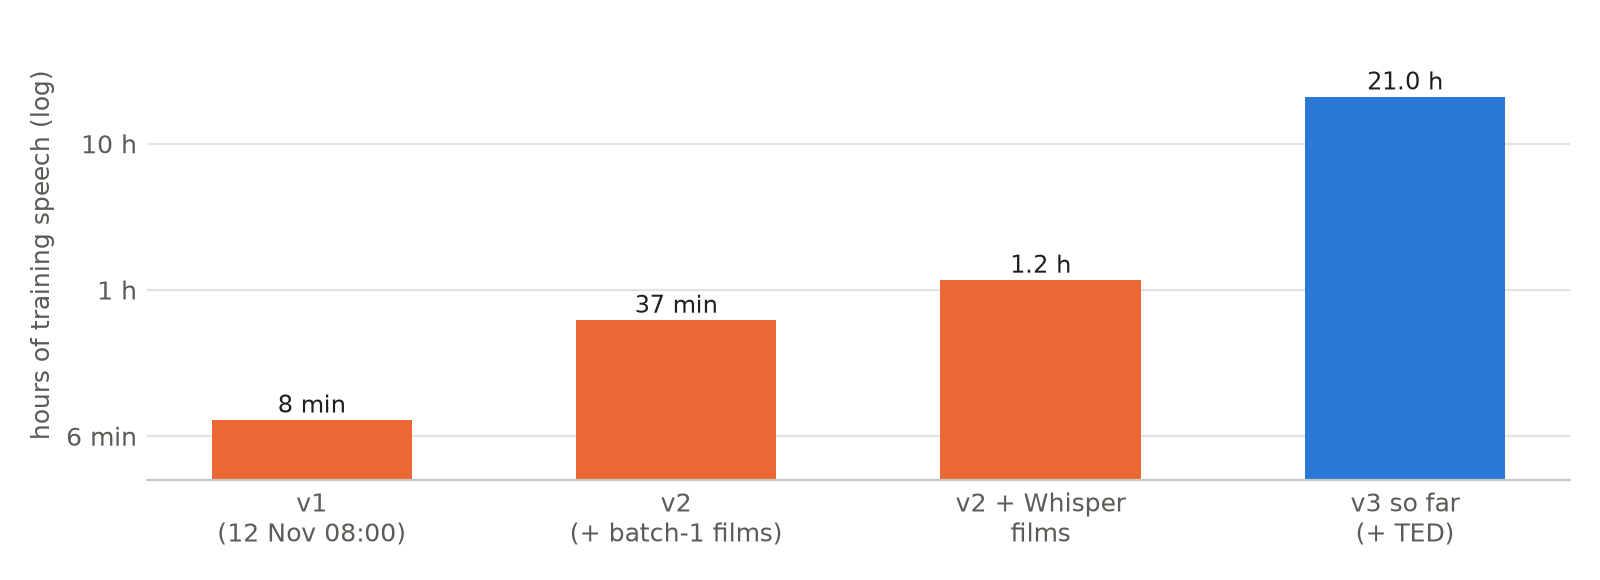
\includegraphics[width=0.86\textwidth]{figures/fig_data_growth.png}
\caption{Labelled out-of-domain training speech per version (log scale). At 19:34 on 12 Nov the
harvester had mined 1,878 of the 3,040 talks: 29,455 clips (20.3\,h).}
\label{fig:growth}
\end{figure}

At the time of writing the harvester had processed 399 hours of TED video. It is on course
for $\approx$39,000 clips ($\approx$27\,h), roughly 150 times this morning's data.

\subsection{The v3 experiment}
\begin{enumerate}
  \item \textbf{Data:} v2 + Whisper films + the full TED harvest. v3 starts automatically when
  the harvester writes its ``finished'' marker.
  \item \textbf{All 11 ResNet variations again}, now on $\sim$40,000 clips, for \textbf{60 epochs
  each} as for our GRID models, with patience raised to 20. Fine-tuning a large encoder usually
  pays off only with enough data. Re-running every variation tells us whether the small-data
  ranking holds.
  \item \textbf{The winner, trained three times} (seeds 1--3, 60 epochs, no early stopping), to
  report a mean and a spread, not a lucky run.
  \item \textbf{Scored once} on the film test, the held-out TED talks, and with the word grammar.
\end{enumerate}
At roughly 5--7 hours per variation this takes \textbf{3--4 days} on the shared Alienware. It
runs unattended: every stage resumes after an interruption, and a boot script restarts the
harvester and the chain if the machine reboots.

\paragraph{What we expect, and how we will judge it.}
Even at $\sim$27 hours we are below the hundreds of hours behind published open-vocabulary
results, so fluent film captions are not expected. Success means three things:
\begin{itemize}
  \item a clear drop in letter errors on the unchanged film test;
  \item many more correct words, especially with the word grammar;
  \item good performance on the held-out TED talks, where the conditions are clean.
\end{itemize}
Comparing each variation on 1.1k vs 40k clips will also show whether the eyes benefit from
more data, which is the question behind Figure~\ref{fig:resnet}.

% =====================================================================
\section{The Demo}
\code{demo/} contains a one-page web app and a FastAPI backend on the Alienware. You press
Record, speak to the phone or laptop camera, and within 2--3\,s see:
\begin{itemize}
  \item the caption;
  \item a bar showing how much Model~P trusted \textbf{sound vs lips}, read directly from the
  fusion gate;
  \item the mouth crops the model actually used.
\end{itemize}
It reuses the evaluation chain (\code{lipscribe.app.inference}), so the demo gives the same
caption as \code{evaluate.py}. It was demonstrated from a phone through a Cloudflare tunnel, which
is now switched off. \code{demo/README.md} explains how to bring it back.

Figure~\ref{fig:demo} shows two real runs of the page. A held-out GRID test speaker (s24, never
used for training) was fed to Chrome as its camera and microphone. We pressed Record, and the clip
was captioned by the backend on the Alienware.

\begin{figure}[htbp]
\centering
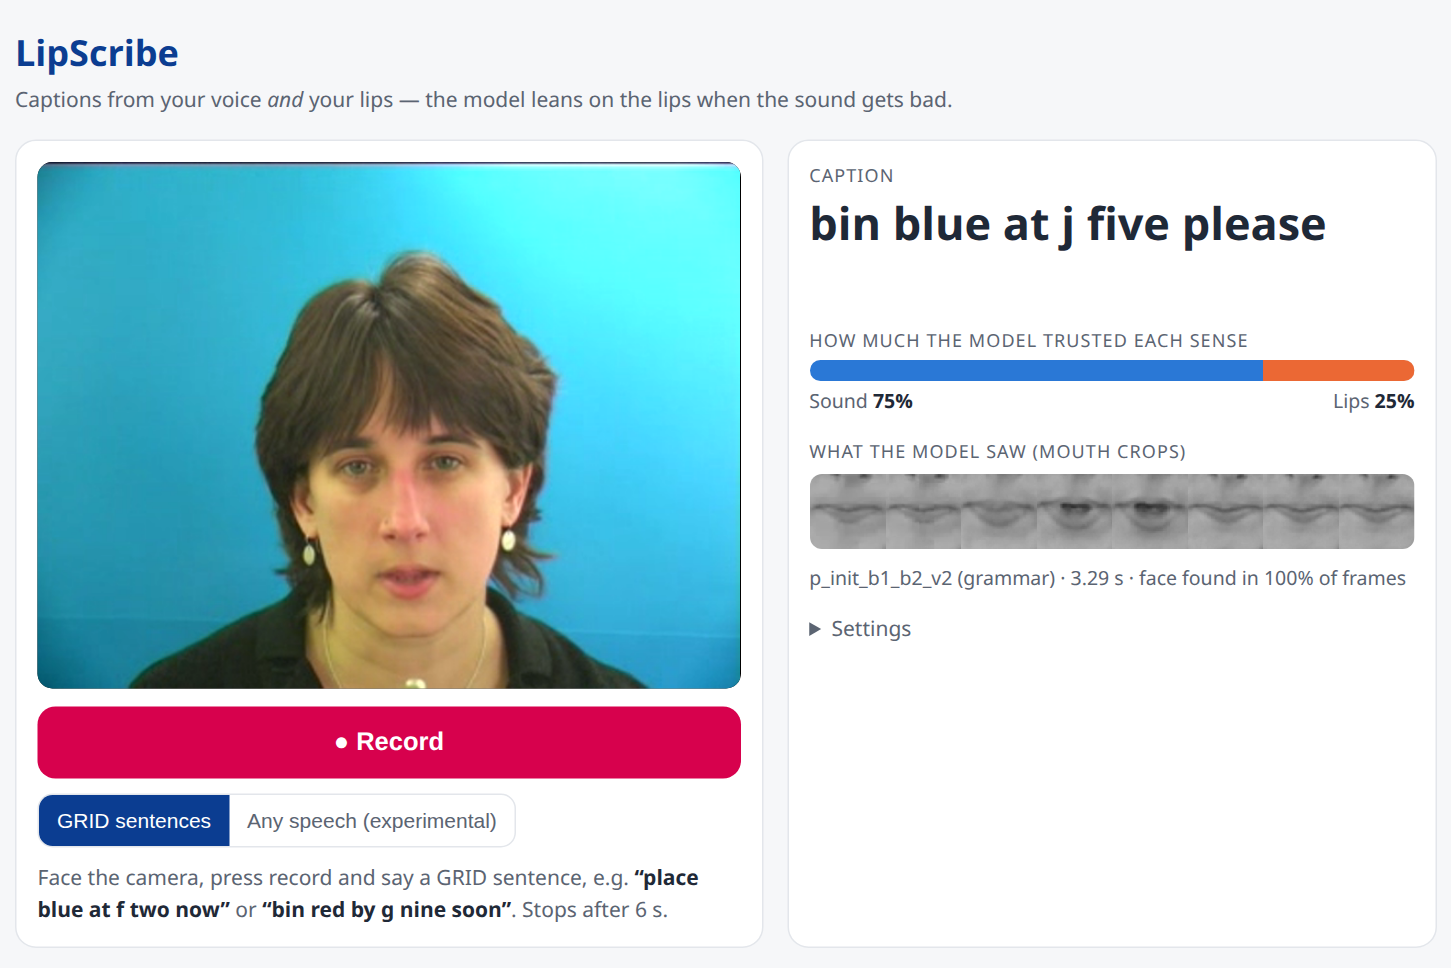
\includegraphics[width=0.495\textwidth]{figures/demo_grid.png}\hfill
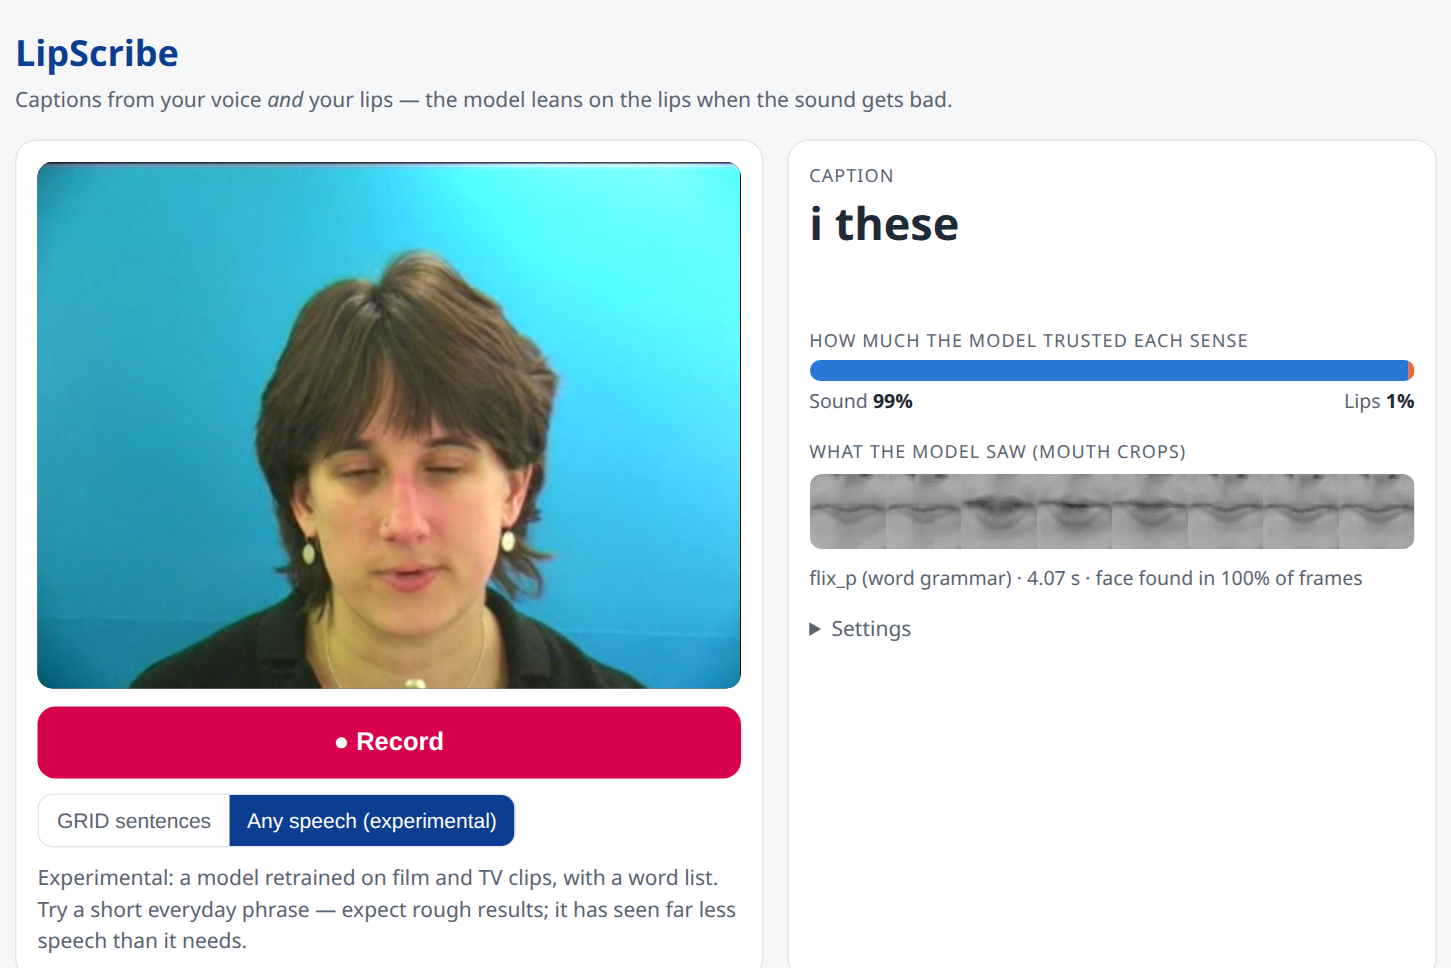
\includegraphics[width=0.495\textwidth]{figures/demo_films.png}
\caption{Screenshots of the web demo. \textbf{Left:} \emph{GRID sentences} mode (P4 + GRID
grammar) writes \textbf{``bin blue at j five please''}, exactly the spoken sentence, in 3.3\,s.
The face was found in 100\,\% of frames, and the model gave the lips 25\,\% of the trust (clean
audio). \textbf{Right:} \emph{Any speech (experimental)} mode on the same clip writes ``i these'':
the film-trained model has forgotten GRID (Table~\ref{tab:flix}) and leans almost entirely on the
sound (lips 1\,\%).}
\label{fig:demo}
\end{figure}

% =====================================================================
\section{Lessons Learned}
\begin{enumerate}
  \item \textbf{In-domain accuracy is not generalisation.} 0.71\,\% WER on GRID and $\approx$100\,\%
  on films describe the \emph{same} model. A test set must reflect where the system will be used.
  \item \textbf{Data dominates.} Every architecture and decoding change this week moved film
  results by a few points. Each step up in data moved letter accuracy steadily.
  \item \textbf{Choose metrics that can still move.} When WER saturates, CER and ``new words
  correct'' carry the signal.
  \item \textbf{Freeze the test set, tune on validation, test once.} We kept the film test fixed
  across every version, so all rows of Table~\ref{tab:flix} are comparable.
  \item \textbf{Engineering is half the work.} Memory limits, stalled pools, slow networks and
  missing tools cost more time today than modelling did. Watchdogs and resumable jobs paid for
  themselves.
  \item \textbf{Legitimate data only.} Using licensed TED talks instead of downloaded films kept
  the project defensible, and it also happens to be better data.
\end{enumerate}

% =====================================================================
\section{Next Steps (Weeks 4--5)}
\begin{enumerate}
  \item \textbf{v3 on TED} (running, $\sim$Monday): report all 11 variations, the 3-seed winner,
  film and TED test results.
  \item \textbf{Merge W3-08} (MFCC + log-Mel features) and retrain Model~P on GRID with it.
  \item \textbf{Gate and attention visualisation} (W4-06) for the report and the demo.
  \item \textbf{Demo:} live captions while speaking (sliding 3\,s window), a fixed public address,
  and the v3 model as the ``any speech'' option.
  \item \textbf{Merge PR \#56} (presentation, Flix pipeline, demo) after team review.
\end{enumerate}

% =====================================================================
\appendix
\section{Glossary}
{\small
\begin{description}[itemsep=2pt]
  \item[WER / CER] Word / character error rate: (substitutions + deletions + insertions) divided by
  the number of reference words / characters. It can exceed 100\,\% when the model adds words.
  \item[CTC] Connectionist Temporal Classification: lets the model output one symbol (or a gap) per
  frame without knowing where each letter starts. A fresh CTC head first outputs only gaps.
  \item[Greedy / beam / grammar decoding] Most likely symbol per frame / several candidate prefixes
  kept at once / only sentences allowed by a pattern.
  \item[Word grammar (lexicon + LM)] Beam search restricted to known words, scoring each word by
  how likely it is to follow the previous one (bigram language model).
  \item[Domain shift] Difference between training and deployment data (studio vs films).
  \item[Overfitting] Memorising the training set; training error falls while validation error rises.
  \item[Transfer learning] Reusing weights learned on one task or dataset as the start for another.
  \item[Pseudo-labels] Labels produced by another model (here Whisper) instead of by people.
  \item[Validation vs test] Validation picks settings and checkpoints; the test set is scored
  once, at the end, so it is never tuned on.
  \item[Seed] The random starting point of a run; repeating with seeds 1--3 shows how much a
  result depends on luck.
\end{description}
}

\end{document}
